\documentclass[11pt,a4paper]{article}
\usepackage[utf8]{inputenc}
\usepackage[english]{babel}
\usepackage[T1]{fontenc}
\usepackage{amsmath}
\usepackage{amsfonts}
\usepackage{amssymb}
\usepackage{graphicx}
\usepackage{array}
\usepackage{multirow}
\usepackage[left=2cm,right=2cm,top=2cm,bottom=2cm]{geometry}
\author{Guillem Tocabens}
\title{First measurements}
\begin{document}

\section{Theory and background} \label{theory}

\section{Scanning system}

\subsection{Aim of the setup}

The main goal of the scanning station is to be able to scan a crystal in all the directions in space. For this to be achieve, the scanning process will be performed measuring coïncidences between the crystal and LYCCA (ref) modules surrounding it. This technique allows to determine where the interaction took place in the crystal in the vertical direction while the radioactive beam is collimated on top of the crystal and moved in order to scan it on a horizontal plane. This way, the crystal can be scanned in all directions in space to allow optimizing the analysis routine afterwards. The station was build starting from zero and trying to match as good as possible the requirements and minimize the risks of any breakdown of the system. The final idea of the setup is presented on Figure~\ref{3D_total} where a 3D drawing of what it should look like is presented. This section of the reports thus concentrates on explaining the approach of building the entire scanning station layer by layer.

\begin{figure}[!h]
\centering
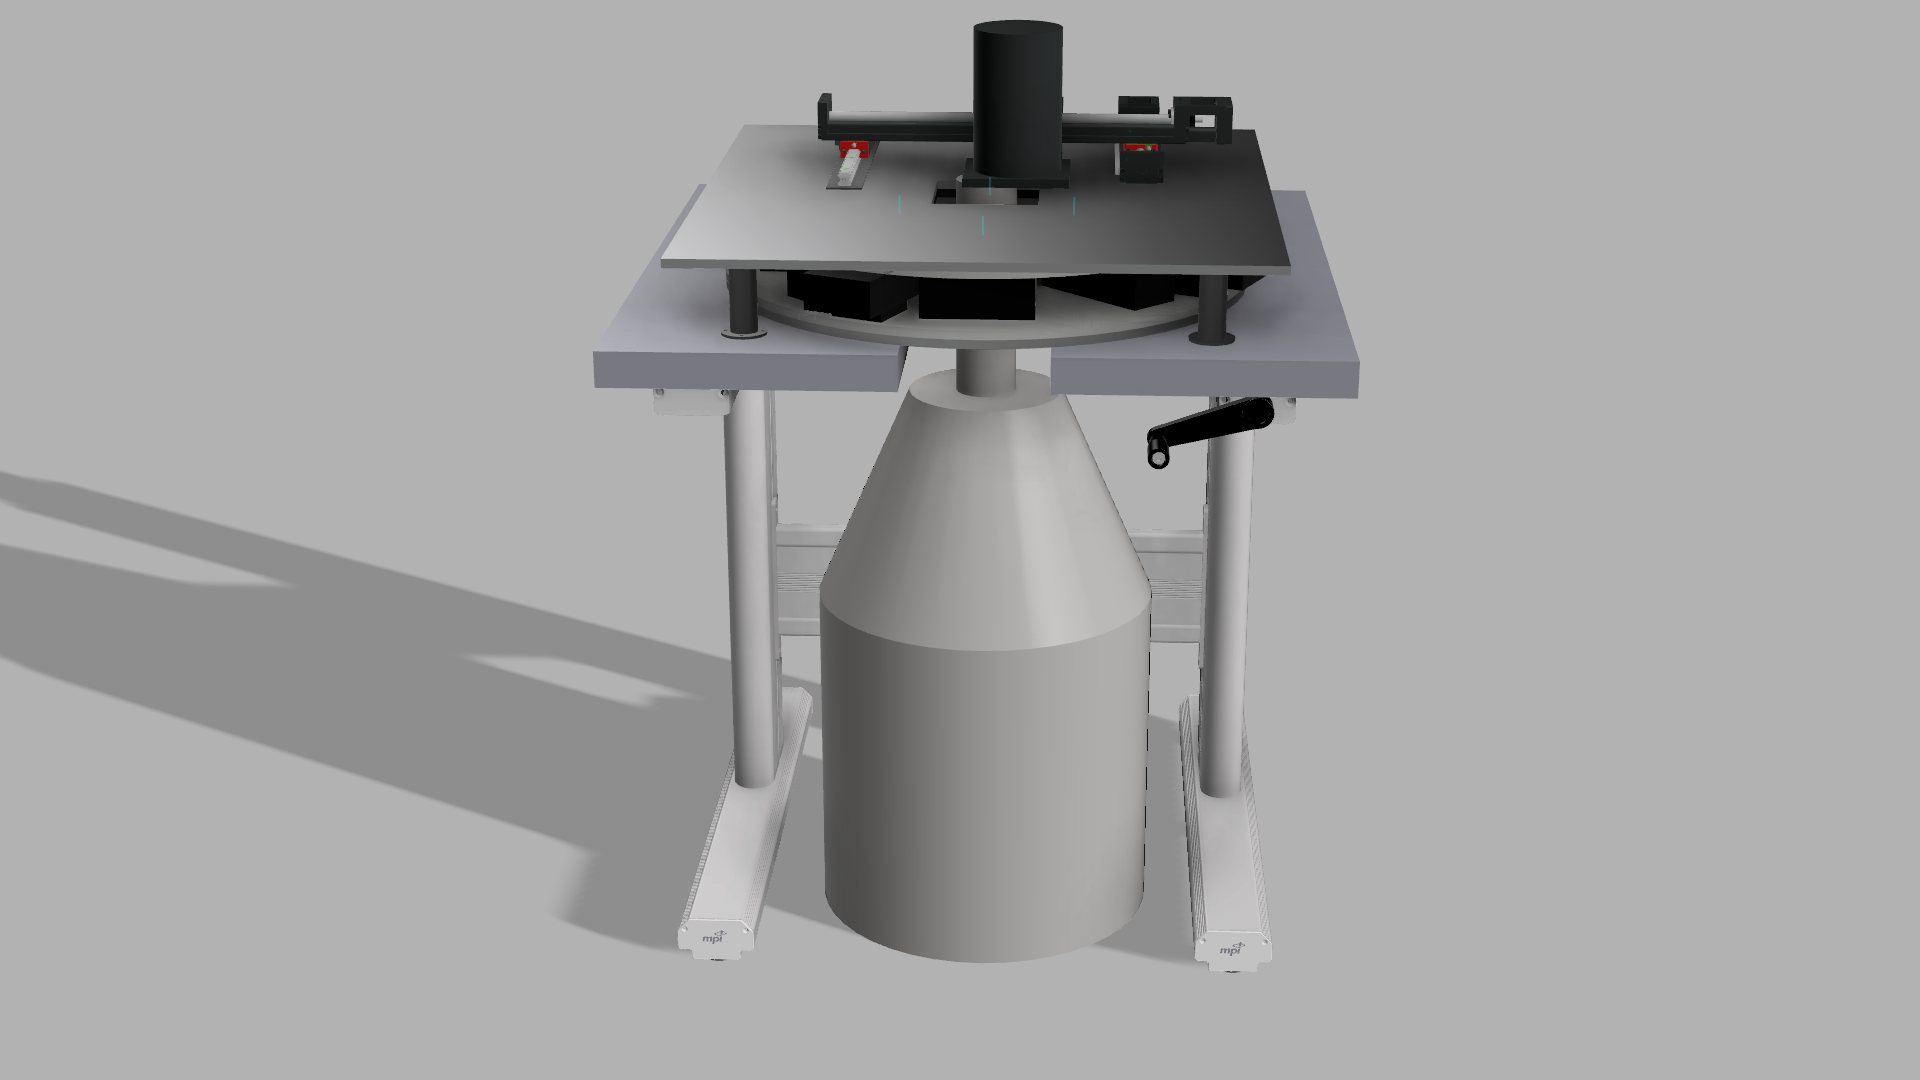
\includegraphics[scale=0.2]{final_setup.png}
\caption{3D view of the final scanning station. From top to bottom are shown the x-y scanning system with the collimator (black cylinder), the LYCCA ring (coïncidence setup) between the top table and the adjustable table and finally the dewar holding the crystal in its upper part (white cylinder).}
\label{3D_total}
\end{figure}

\subsection{Coïncidence setup} \label{coin_setup}

The coïncidence setup is made of a ring containing 12 LYCCA module (ref) surrounding the crystal to determine the height where the interaction took place in it. Horizontal absorbers made of tungsten are placed between the crystal and the modules to enable only some coïncidences to be detected in the zones between two absorbers (see Figure~\ref{coïncidence}). The crystal is placed in the middle of the ring and the collimated beam is directed from above towards the crystal.

ADD FIGURE OF LYCCA/ABSORBERS

This part of the setup was the only part already built up that did not need to be designed.

\subsection{The holding structure}

This part of the setup was rather complicated to develop while some major constraints have to be taken into account. The first constraint is that the dewar must fit under the table while the crystal must be protruding above its plate to allow the coïncidence setup to be mounted on the table. The solution here was to design a table with a hole in the middle allowing this as can be seen on the final design of the table, Figure~\ref{table}. Another constraint was to have a height adjustable table. Indeed, the coïncidence setup could not cover the whole crystal to be scanned in height, having a height adjustable support for it could make a scan on the whole vertical direction of the crystal possible.

Finally, the loading capacity of the table should be sufficiently high while some pieces such as the absorbers (\ref{coin_setup}) or the collimator are made of tungsten for a global weight of around 60 to 70 kilograms, without counting other pieces, the total weight being estimated around 100 kilogramms. A 3D view of the table is shown on Figure~\ref{table}. On this first layer, the LYCCA ring will be mounted in the middle to match with the end of the cap coming from the dewar.

ADD 3D VIEW OF THE TABLE + TOP PLATE ONLY

The next step was thus to find a solution in order to put the x-y scanning system on top of the table. Again, this second layer should be quite resistant while a load of around 30 kilograms would then be added on top of it. In order for the directed beam to reach the crystal, a hole should be drilled in the middle of the top plate, matching the dimensions of the crystal to scan. As the bottom table is already height adjustable, this second layer did not need to be as well, reducing the constraints. For all these reasons, a thick plate of iron with a square hole in the middle was designed to be mounted on four legs fixed on the table in the four corners. The result presenting the structure of the setup is shown on figure~\ref{table}.

\subsection{The x-y scanning system}

After the global structure of the scanning station was decided, certainly the most critical step was to develop the x-y scanning system. Indeed, this construction had to fulfill several conditions such as a rather good uncertainty on the positionning, the possibility to remote control the movement, a quite high load capacity, etc. After a few research and calls to different companies, the best option seemed to use two linear units and a linear guide and hang the collimator containing the source on one of them (see Figure~\ref{scan}). Linear units are devices that contain a rail and a wagon and use a screw going through the wagon to move it with a motor. Thus, a linear unit can move its wagon in one given direction. Thus, fixing two of those units on one another and perpendicular to each other should allow an object fixed on top to move in two different directions. The linear guide, which has basically the same role as the linear units except it is not motorized and then just follows the lead, is placed parallel to the first linear unit so that the one on top can be fixed to both, increasing the stability and load capacity of the construction.

The whole scanning system needs to be mounted on top of the principal structure so that the radioactive beam can be directed towards the crystal. As the linear units and the linear guide have holes, matching holes were drilled in the top plate at the correct positions in order to be able to cover the square hole in the middle of the plate. The last concerns about the units were to obtain a correct precision in their movement and to be sure that they could hold the collimator. The precision is only limited by the motors used to move the wagons, while the inner precision of the units is of the order to some microns, way better than what is needed here, as $0.1~mm$ seems reasonable. Thus the motors were chosen to match this requirement and to be powerful enough to push the wagon with the collimator (around $26~kg$). For the load, the linear units are not supposed to hold a great vertical load, but they can support a high torque in any direction. An arm protruding from the top unit was then designed to hold the collimator. This would minimise the vertical load applied on the wagon and maximise the torque, making this solution viable.

The collimator arm was the last piece of the setup to be designed and its ideal shape was quite hard to determine. The first thought was to build it as a stair, with the upper step being fixed on the wagon and the lower one holding the collimator. As the collimator is quite imposant and extremely dense (tungsten alloy to collimate the beam in a $1~mm$ hole going through it), a back up plan was designed using two spherical wheels on an extension of the arm that would allow the collimator to rest on the top plate, reparting the load on it (see Figure~\ref{arm}). To study the need for this extension, stress simulations were performed for two principal materials, aluminum and steel. The results, estimated for a load of $30~kg$ applied on the whole lower step, showed a maximum vertical deformationof around $0.3~mm$ for aluminum and $0.1~mm$ for steel. Such a deformation would lead to an uncertainty on the position of the beam on the crystal of $0.1~mm$ and $0.05~mm$ using aluminum and steel respectively. The solution that was kept was thus a steel arm, as shown on Figure~\ref{arm} and the back up plan with the extension was still kept in mind if the first tests with the regular arm were not satisfying.

\subsection{Final adjustments and building of the station}



\section{Scanning the prototype detector}

While the scanning station was not already built and the different pieces took several months to arrive in Lund, measurements were performed with another setup that used material available in Lund. This was made to verify the measurements of resolution given by the company building the prototypes of detector, Canberra. These first measurements were also an opportunity to study the effect of capacitance of the detector and trapping on the resolution and compare both effects.

\subsection{Overall setup} \label{setup}

The setup uses three detectors: two scintillator detectors, placed on the sides (black squared boxes in Figure \ref{Setup}) and one semiconductor detector - hyperpure germanium detector - below the collimated source (grey cylinder in Figure \ref{Setup}). The source is placed on the top lead brick which contains a hole in the middle to collimate the radioactive source. In that position, the source is 97mm from the top of the crystal, which is 5mm from the top of the cryostat, and collimated in a 5mm hole through an 80mm lead brick. The source is covered by a little lead brick and the setup is shielded by lead to avoid propagation of gamma radiation away from the setup (see Figure \ref{Setup_front}).

\begin{figure}[!h]
\centering
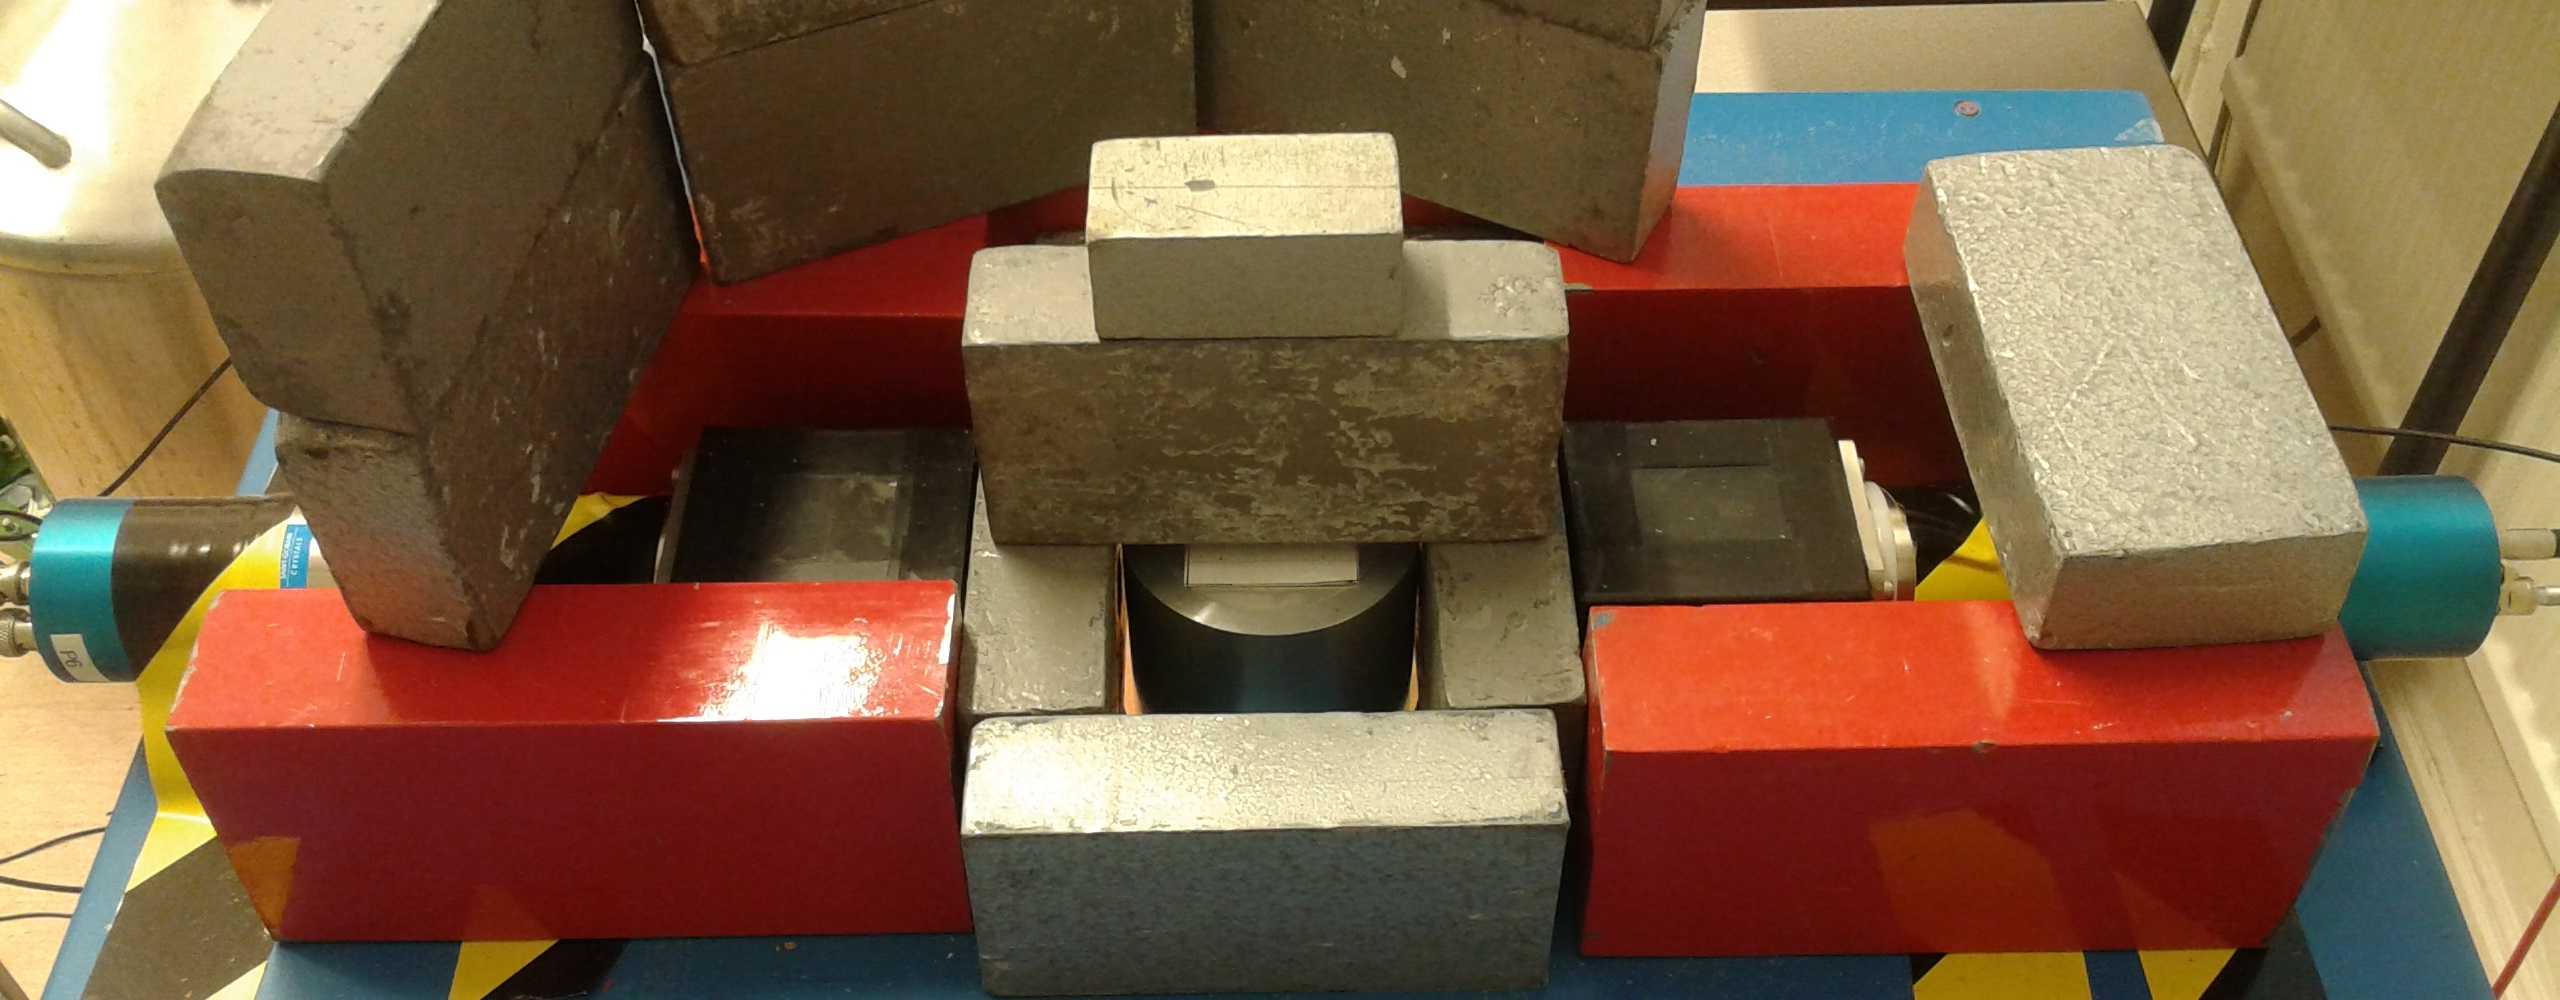
\includegraphics[scale=0.15]{New_setup_back.jpg}
\caption{Back of the original setup. The scintillator detectors are the black squared boxes on the sides of the germanium detector, placed in a cryostat (grey cylinder in the middle).}
\label{Setup}
\end{figure}

\begin{figure}[!h]
\centering
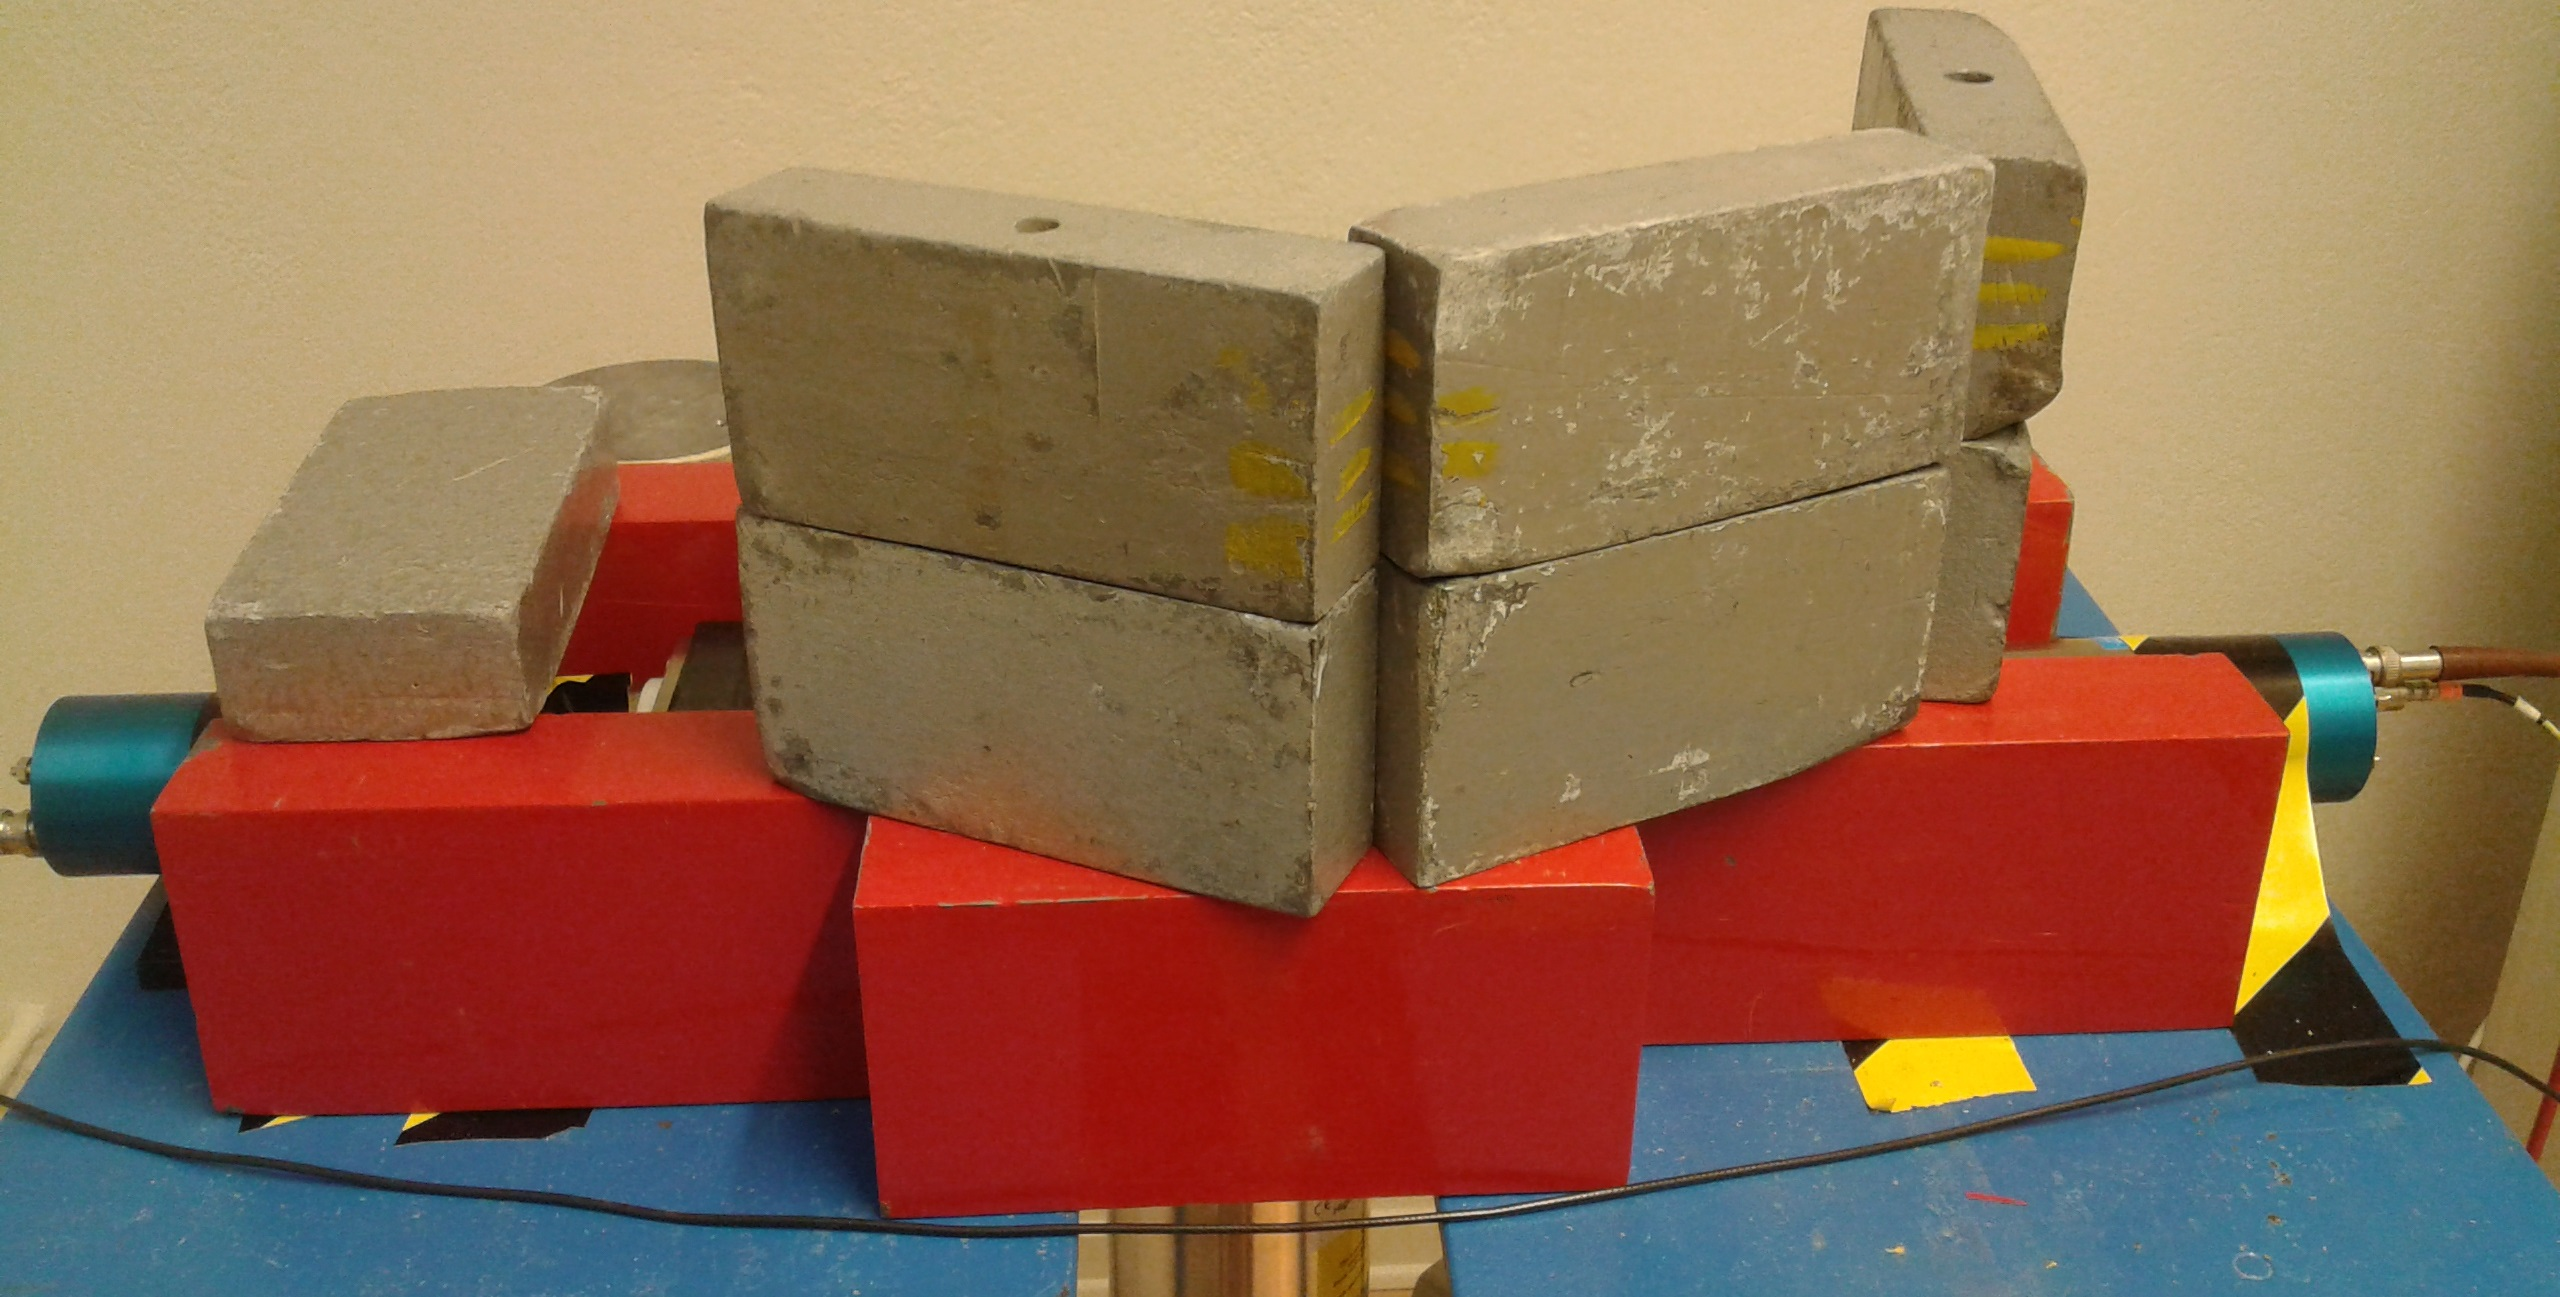
\includegraphics[scale=0.15]{New_setup_front.jpg}
\caption{Front side of the original setup (with the lead shielding). Two holed lead bricks can be seen on this picture as the one used to obtain a collimated beam.}
\label{Setup_front}
\end{figure}

\subsection{Process of measurement} \label{protocol}

For the first set of measurements, only the germanium detector was used but not the scintillator detectors. The goal of this experiment was to determine some spectral properties of the detector depending on the location of the collimated source such as the resolution of the crystal. Therefore, the source was directed onto five different points on the top of the crystal: one measurement was performed directing the beam in the center of the crystal surface, and four in the corners of the crystal surface. This was made possible by the use of a holed lead brick on top of which the source was positioned. The scanning was conducted as described below and two different cobalt sources were used, one of $^{60}$Co and one of $^{57}$Co.

In the case of $^{60}$Co, the source was held in one of the positions until the net area\footnote{In the analysis of the spectra, two areas need to be differenciated~: the total area, which gives the total number of counts between two channels, and the net area, which gives the number of counts between two channel substracted by the background.} of the studied peak (peak at $1332~keV$) contained at least 100~000 counts to match the measurement performed by the company manufacturing the detectors. Since the $^{57}$Co source was much less active, the measurement was stopped when the net area of the studied peak (peak at $122~keV$) contained around 1~000 counts.

The very first step was to perform the calibration. To do so, the two lines present in the spectrum of $^{60}$Co were used (lines at $1173~keV$ and $1332~keV$) and associated to a channel in the 8192 channel analyzer. In order to avoid a shift in the low energy range, the line at $122~keV$ in the spectrum of $^{57}$Co was also used. Then a linear fit was performed to get the the calibrated energies and then the equation of channels as a function of energy that was used in the analysis procedure later on (the data analysis is described in section~\ref{analysis}).

\subsection{Electronics}

For the first set of measurements, the scintillator detectors and the coincidence setup were not used, thus the electronics are relatively simple. The germanium detector is powered by a high voltage supply as explained in section~\ref{theory}. After going through a preamplifier, included in the cryostat, the signal is sent to an amplifier. Besides amplifying the signal, the amplifier also shapes it to a Gaussian. It is then digitized by an Analog to Digital Converter, ADC, and a multichannel analyzer sorts the digital values which are sent to the computer that collects the data using the Maestro software. Both the high voltage supply and the amplifier are Nuclear Instrumentation Modules (NIM, a standard set of modules) and are placed in a NIM crate that provides the necessary power for operation.

\subsection{Results and analysis} \label{analysis}

\subsubsection{First prototype}

The measurements that were conducted here had two main objectives. First, they were done in order to verify the values of the principal characteristics claimed by Canberra but this first experiment was also performed to get a first idea of how the crystals will be scanned with the final scanning system and what quantities to measure. This way, the detector was scanned following the protocol explained in section~\ref{protocol}.

The resolution of the detector, given by the full width at half maximum (FWHM), along with the shape of the peak, emphasized by the ratios between, the full width at tenth and fiftieth maximum, and the FWHM, were studied. The results are shown in the two tables below, both for the $^{60}$Co and $^{57}$Co source (Figure~\ref{recap}). For each source, the peaks in the spectra were fitted with Gaussians and the FWHM was deduced from the fit. As the fitting program uses the FWHM to optimise the fit, the value given by the Gaussian is the same as the real value that can be read from the data. This is not the case when it comes to the FWTM and FWFM and these values were directly read off the spectra without using the fit.

\begin{figure}[!h]
\centering
\caption{Recap charts of the obtained results using the $^{60}$Co and $^{57}$Co sources. $^{60}$Co and $^{57}$Co were used for calibration to avoid possible shifts in the low energy range.}
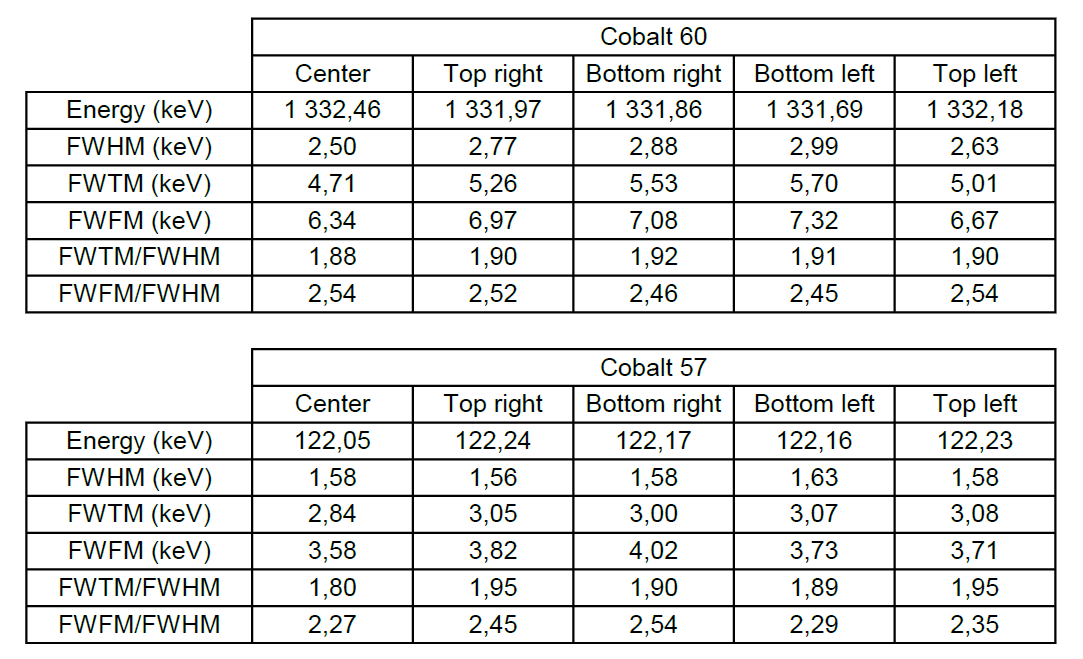
\includegraphics[scale=0.6]{Scan_Cos_2.png}
\label{recap}
\end{figure}

The very first thing we can notice in this set of measurments is that there is a shift in energy depending on where the beam was collimated. This shift in energy between the expected values (\cite{lit}) and the measured values goes up to around $0.8~keV$ if the beam is not directed towards the center of the crystal. It is normal that the measure of the peak energy in the center of the crystal is the closest to the energy we can find in the literature, while the calibration was made using this measurement and the measurement in the center with a $^{57}$Co source. This is also why the same measurement done in the center of the crystal with the $^{57}$Co source gives the closest result to the literature (TOPPED CORRECTIONS HERE) value. The shift in energy is more important in the range of high energies and thus for the results obtained with the $^{60}$Co source. This is not an observation that is really possible to explain, but the fact that the peaks are not seen at the same energy depending on where the beam is directed is still interesting to notice. As stated in different articles treating the subject, this could come from the difference of path the charge carriers need to travel depending if the interaction happens in a corner or in the center of the crystal. Indeed, as seen before in section~\ref{theory}, the more charge carriers have to travel to reach the electrodes and be collected, the more they are susceptible of being trapped in the crystal. This can imply a shift in energy and also differences in the measure of the resolution of the crystal as explained earlier.

The same observation can be done while looking at the resolution measured in the different parts of the crystal. As for the peak energy, the difference is not huge for measurements with the $^{57}$Co source. But for the second cobalt source, the resolution varies from $2.50~keV$ up to $2.99~keV$ which is quite a big difference. Nonetheless, these values of resolution are roughly in agreement with the values provided by Canberra for the $^{60}$Co, which were, for this first prototype, of $2.40~keV$ at $1332.5~keV$. The difference between both measurements in Lund and in Canberra can be explained by the different experimental conditions in which the measurements were done. The cryostat used with the crystal could influence the measured resolution, as welle as the electronics and the treatment protocol of the data. While the first is not critical, an improvement in the electronics used can change the values of the resolution by quite a lot and as the program used to analyse the data was not the same in both cases, this could also influence the measured FWHM. The real problem here is the huge difference between the resolution obtained at Lund and at Canberra for the $^{57}$Co source~: $1.59~keV$ were measured in Lund and $0.81~keV$ which means almost twice what the final goal is. This could be explained by the $^{57}$Co source used in Lund~: the source was too weak and the net area of 100~000 counts under the peak recommended by Canberra could not be reached. These values were measured with a net area of around 1~000 counts under the peak which was thus not pointing as high over the background as it should have.

Finally, the symmetry ratios have been calculated and compared to the values given by Canberra. Again, for the $^{57}$Co source, it may not make a lot of sense to look at those values, as the peak is not large enough to be analyzed in a proper way. The values obtained for the $^{60}$Co source are closer to the theoretical values than the values given by Canberra ($1.90$ and $2.50$ against $2.19$ and $ $), indicating that the peaks obtained on the spectra have a better Gaussian shape.

\subsubsection{Second prototype}

For the second prototype, the goal was just to do the measurements to check the values provided by Canberra for this prototype and the detector was not scanned as the first prototype. Instead, the source was just placed at the exact same distance from the cap as described in~\ref{setup} but not collimated using a lead brick, in order to get a proper number of counts per second. Results are shown in chart~\ref{recap2} for the different sources that were used.

\begin{figure}[!h]
\centering
\caption{Comparative chart of the obtained resolution using, from left to right, $^{241}$Am, $^{57}$Co, $^{60}$Co and $^{137}$Cs. $^{60}$Co and $^{57}$Co were used for calibration to avoid possible shifts in the low energy range.}
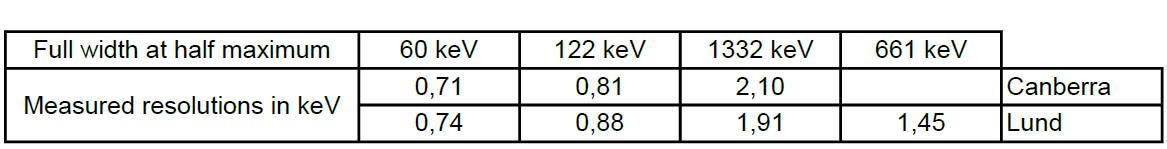
\includegraphics[scale=0.6]{result_2.png}
\label{recap2}
\end{figure}
Here the main focus was the measure of the resolution that should match the values given by Canberra (except for the cesium source, which was just performed to have a value of resolution in that range of energies). In the three cases that were given by Canberra, the results were in agreement and there was no critical measures like it was the case with the first crystal. The low energy resolution was found to be way higher than the one from the first crystal and overall the resolution increased quite significantly compared to the other detector. As for the first tested prototype, all these results are to be optimised using better electronics and cryostat as well as optimising the data analysis routine.

The shape factors of the peaks were also determined and matched quite well the ones given by the company, again slightly better than the ones from the first crystal (Figure~\ref{shape2}). The difference between these values can also be explained by the use of different electronics, that could lead to a better peak shape even if the differences are not significantly high.

\begin{figure}[!h]
\centering
\caption{Comparative chart of the peak shape at $1332.5~keV$ from the $^{60}$Co spectrum.}
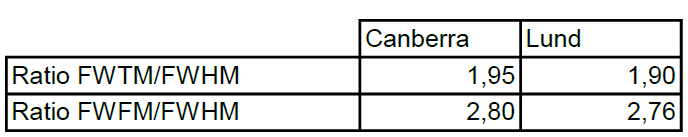
\includegraphics[scale=0.7]{shape.png}
\label{shape2}
\end{figure}
These results are quite interesting to analyse because the main difference between both crystals is the length of the hole in the middle, which is longer for the second prototype. What is important here is that the capacitance of the crystal increases with the length of the hole and thus, the resolution should decrease as the hole gets longer (see section~\ref{theory}). This is nonetheless not the case and the behaviour looks exactly the opposite, while the resolution increased with the second crystal. One of the reasons for that could be that as the length of the hole is increasing, the mean path of the charge carriers to travel to the inner electrode is decreasing and thus trapping is getting less important. As discussed earlier, effects of trapping can be really important on both the count rate and the resolution of the detector. From these results it could even be said that effects of trapping are much more important than capacitance as resolution was better for the second prototype. Trapping is also a big problem when it comes to the shape of the peak, which again confirms the fact that trapping was affected by the length of the hole and that a longer hole is better to obtain a good resolution in a semi-conductor detector. Finally, the quality of the crystal, which is not provided by the company, could highly affect the resolution of the detector and the first crystal may have been worse than the second one, also explaining the differences in resolution obtained.

\end{document}